\documentclass[10pt,oneside]{article}
\usepackage[T1]{fontenc}
\usepackage[utf8]{inputenc}
% \usepackage{lmodern}
%\usepackage[adobe-utopia,uppercase=upright,greeklowercase=upright]{mathdesign}
\usepackage[adobe-utopia]{mathdesign}
%\usepackage{minionpro}
% \usepackage{pifont}
% \usepackage{amssymb}
\usepackage{amsmath}
\usepackage[francais]{babel}
% \usepackage[francais]{varioref}
\usepackage[dvips]{graphicx}

\usepackage{framed}
\usepackage[normalem]{ulem}
\usepackage{fancyhdr}
\usepackage{titlesec}
\usepackage{vmargin}
\usepackage{longtable}

\usepackage{ifthen}


%\usepackage{epsfig}
\usepackage{subfig}

\usepackage{multirow}
\usepackage{multicol} % Portions de texte en colonnes
\usepackage{flafter}%floatants après la référence



\usepackage{color}
\usepackage{colortbl}


\definecolor{gris25}{gray}{0.75}
\definecolor{bleu}{RGB}{18,33,98}
\definecolor{bleuf}{RGB}{42,94,171}
\definecolor{bleuc}{RGB}{231,239,247}
\definecolor{rougef}{RGB}{185,18,27}
\definecolor{rougec}{RGB}{255,230,231}
\definecolor{vertf}{RGB}{103,126,82}
\definecolor{vertc}{RGB}{220,255,191}
\definecolor{violetf}{RGB}{112,48,160}
\definecolor{violetc}{RGB}{230,224,236}

\newenvironment{sci}[1][\hsize]%
{%
    \def\FrameCommand%
    {%
%\rotatebox{90}{\textit{\textsf{Scilab}}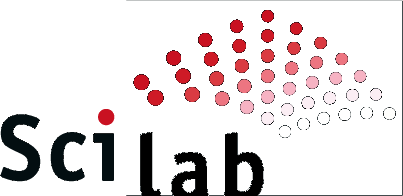
\includegraphics[height=.8cm]{png/logo_scilab}} 
\rotatebox{90}{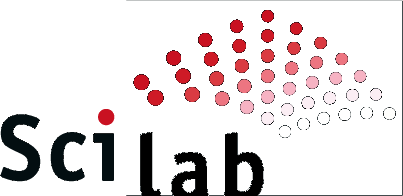
\includegraphics[height=.6cm]{png/logo_scilab}} 
        {\color{violetf}\vrule width 3pt}%
        \hspace{0pt}%must no space.
        \fboxsep=\FrameSep\colorbox{violetc}%
    }%
    \MakeFramed{\hsize #1 \advance\hsize-\width\FrameRestore}%
}%
{\endMakeFramed}%

\newenvironment{pseudo}[1][\hsize]%
{%
    \def\FrameCommand%
    {%
\rotatebox{90}{\textit{\textsf{Pseudo Code}}} 
        {\color{violetf}\vrule width 3pt}%
        \hspace{0pt}%must no space.
        \fboxsep=\FrameSep\colorbox{violetc}%
    }%
    \MakeFramed{\hsize #1 \advance\hsize-\width\FrameRestore}%
}%
{\endMakeFramed}%

\newenvironment{py}[1][\hsize]%
{%
    \def\FrameCommand%
    {%
%\rotatebox{90}{\textit{\textsf{Python}}} 
\rotatebox{90}{
\includegraphics[height=.6cm]{png/logo_python}} 
        {\color{violetf}\vrule width 3pt}%
        \hspace{0pt}%must no space.
        \fboxsep=\FrameSep\colorbox{violetc}%
    }%
    \MakeFramed{\hsize #1 \advance\hsize-\width\FrameRestore}%
}%
{\endMakeFramed}%


\newenvironment{corrige}[1][\hsize]%
{%
    \def\FrameCommand
    {%
\rotatebox{90}{\textit{\textsf{Correction}}} 
        {\color{violetf}\vrule width 3pt}%
        \hspace{0pt}%must no space.
        \fboxsep=\FrameSep\colorbox{violetc}%
    }%
    \MakeFramed{\hsize#1\advance\hsize-\width\FrameRestore}%
}%
{\endMakeFramed}%



\newenvironment{rem}[1][\hsize]%
{%
    \def\FrameCommand
    {%
\rotatebox{90}{\textit{\textsf{Remarque}}} 
        {\color{bleuf}\vrule width 3pt}%
        \hspace{0pt}%must no space.
        \fboxsep=\FrameSep\colorbox{bleuc}%
    }%
    \MakeFramed{\hsize#1\advance\hsize-\width\FrameRestore}%
}%
{\endMakeFramed}%


\newenvironment{savoir}[1][\hsize]%
{%
    \def\FrameCommand
    {%
\rotatebox{90}{\textit{\textsf{Savoir}}} 
        {\color{bleuf}\vrule width 3pt}%
        \hspace{0pt}%must no space.
        \fboxsep=\FrameSep\colorbox{bleuc}%
    }%
    \MakeFramed{\hsize#1\advance\hsize-\width\FrameRestore}%
}%
{\endMakeFramed}%

\newenvironment{prob}[1][\hsize]%
{%
    \def\FrameCommand%
    {%
\rotatebox{90}{\textit{\textsf{ Problématique}}} 
        {\color{rougef}\vrule width 3pt}%
        \hspace{0pt}%must no space.
        \fboxsep=\FrameSep\colorbox{rougec}%
    }%
    \MakeFramed{\hsize#1\advance\hsize-\width\FrameRestore}%
}%
{\endMakeFramed}%

\newenvironment{obj}[1][\hsize]%
{%
    \def\FrameCommand%
    {%
\rotatebox{90}{\textit{\textsf{Objectifs}}} 
        {\color{rougef}\vrule width 3pt}%
        \hspace{0pt}%must no space.
        \fboxsep=\FrameSep\colorbox{rougec}%
    }%
    \MakeFramed{\hsize#1\advance\hsize-\width\FrameRestore}%
}%
{\endMakeFramed}%

\newenvironment{defi}[1][\hsize]%
{%
    \def\FrameCommand%
    {%
\rotatebox{90}{\textit{\textsf{Définition\\}}} 
        {\color{bleuf}\vrule width 3pt}%
        \hspace{0pt}%must no space.
        \fboxsep=\FrameSep\colorbox{bleuc}%
    }%
    \MakeFramed{\hsize#1\advance\hsize-\width\FrameRestore}%
}%
{\endMakeFramed}%


\newenvironment{demo}[1][\hsize]%
{%
    \def\FrameCommand%
    {%
\rotatebox{90}{\textit{\textsf{Démonstration\\}}} 
        {\color{bleuf}\vrule width 3pt}%
        \hspace{0pt}%must no space.
        \fboxsep=\FrameSep\colorbox{bleuc}%
    }%
    \MakeFramed{\hsize#1\advance\hsize-\width\FrameRestore}%
}%
{\endMakeFramed}%


\newenvironment{hypo}[1][\hsize]%
{%
    \def\FrameCommand%
    {%
\rotatebox{90}{\textit{\textsf{Hypothèse\\}}} 
        {\color{bleuf}\vrule width 3pt}%
        \hspace{0pt}%must no space.
        \fboxsep=\FrameSep\colorbox{bleuc}%
    }%
    \MakeFramed{\hsize#1\advance\hsize-\width\FrameRestore}%
}%
{\endMakeFramed}%


\newenvironment{prop}[1][\hsize]%
{%
    \def\FrameCommand%
    {%
\rotatebox{90}{\textit{\textsf{Propriété\\}}} 
        {\color{bleuf}\vrule width 3pt}%
        \hspace{0pt}%must no space.
        \fboxsep=\FrameSep\colorbox{bleuc}%
    }%
    \MakeFramed{\hsize#1\advance\hsize-\width\FrameRestore}%
}%
{\endMakeFramed}%

\newenvironment{props}[1][\hsize]%
{%
    \def\FrameCommand%
    {%
\rotatebox{90}{\textit{\textsf{Propriétés\\}}} 
        {\color{bleuf}\vrule width 3pt}%
        \hspace{0pt}%must no space.
        \fboxsep=\FrameSep\colorbox{bleuc}%
    }%
    \MakeFramed{\hsize#1\advance\hsize-\width\FrameRestore}%
}%
{\endMakeFramed}%

\newenvironment{exemple}[1][\hsize]%
{%
    \def\FrameCommand%
    {%
\rotatebox{90}{\textit{\textsf{Exemple\\}}} 
        {\color{vertf}\vrule width 3pt}%
        \hspace{0pt}%must no space.
        \fboxsep=\FrameSep\colorbox{vertc}%
    }%
    \MakeFramed{\hsize#1\advance\hsize-\width\FrameRestore}%
}%
{\endMakeFramed}%

\newenvironment{resultat}[1][\hsize]%
{%
    \def\FrameCommand%
    {%
\rotatebox{90}{\textit{\textsf{Résultat\\}}} 
        {\color{rougef}\vrule width 3pt}%
        \hspace{0pt}%must no space.
        \fboxsep=\FrameSep\colorbox{rougec}%
    }%
    \MakeFramed{\hsize#1\advance\hsize-\width\FrameRestore}%
}%
{\endMakeFramed}%

\newenvironment{methode}[1][\hsize]%
{%
    \def\FrameCommand%
    {%
\rotatebox{90}{\textit{\textsf{Méthode\\}}} 
        {\color{rougef}\vrule width 3pt}%
        \hspace{0pt}%must no space.
        \fboxsep=\FrameSep\colorbox{rougec}%
    }%
    \MakeFramed{\hsize#1\advance\hsize-\width\FrameRestore}%
}%
{\endMakeFramed}%

\newenvironment{theo}[1][\hsize]%
{%
    \def\FrameCommand%
    {%
\rotatebox{90}{\textit{\textsf{Théorème\\}}} 
        {\color{rougef}\vrule width 3pt}%
        \hspace{0pt}%must no space.
        \fboxsep=\FrameSep\colorbox{rougec}%
    }%
    \MakeFramed{\hsize#1\advance\hsize-\width\FrameRestore}%
}%
{\endMakeFramed}%

\newenvironment{warn}[1][\hsize]%
{%
    \def\FrameCommand%
    {%
\rotatebox{90}{\textit{\textsf{Attention\\}}} 
        {\color{rougef}\vrule width 3pt}%
        \hspace{0pt}%must no space.
        \fboxsep=\FrameSep\colorbox{rougec}%
    }%
    \MakeFramed{\hsize#1\advance\hsize-\width\FrameRestore}%
}%
{\endMakeFramed}%

% \usepackage{pstricks}
%\usepackage{minitoc}
% \setcounter{minitocdepth}{4}

\setcounter{tocdepth}{2}

% \mtcselectlanguage{french} 

%\usepackage{draftcopy}% "Brouillon"
% \usepackage{floatflt}
\usepackage{psfrag}
%\usepackage{listings} % Permet d'insérer du code de programmation
\renewcommand{\baselinestretch}{1.2}

% Changer la numérotation des figures :
% ------------------------------------
% \makeatletter
% \renewcommand{\thefigure}{\ifnum \c@section>\z@ \thesection.\fi
%  \@arabic\c@figure}
% \@addtoreset{figure}{section}
% \makeatother
 


%%%%%%%%%%%%
% Définition des vecteurs %
%%%%%%%%%%%%
 \newcommand{\vect}[1]{\overrightarrow{#1}}

%%%%%%%%%%%%
% Définition des torseusr %
%%%%%%%%%%%%

 \newcommand{\torseur}[1]{%
\left\{{#1}\right\}
}

\newcommand{\torseurcin}[3]{%
\left\{\mathcal{#1} \left(#2/#3 \right) \right\}
}

\newcommand{\torseurstat}[3]{%
\left\{\mathcal{#1} \left(#2\rightarrow #3 \right) \right\}
}

 \newcommand{\torseurc}[8]{%
%\left\{#1 \right\}=
\left\{
{#1}
\right\}
 = 
\left\{%
\begin{array}{cc}%
{#2} & {#5}\\%
{#3} & {#6}\\%
{#4} & {#7}\\%
\end{array}%
\right\}_{#8}%
}

 \newcommand{\torseurcol}[7]{
\left\{%
\begin{array}{cc}%
{#1} & {#4}\\%
{#2} & {#5}\\%
{#3} & {#6}\\%
\end{array}%
\right\}_{#7}%
}

 \newcommand{\torseurl}[3]{%
%\left\{\mathcal{#1}\right\}_{#2}=%
\left\{%
\begin{array}{l}%
{#1} \\%
{#2} %
\end{array}%
\right\}_{#3}%
}

 \newcommand{\vectv}[3]{%
\vect{V\left( {#1} \in {#2}/{#3}\right)}
}


\newcommand{\vectf}[2]{%
\vect{R\left( {#1} \rightarrow {#2}\right)}
}

\newcommand{\vectm}[3]{%
\vect{\mathcal{M}\left( {#1}, {#2} \rightarrow {#3}\right)}
}


 \newcommand{\vectg}[3]{%
\vect{\Gamma \left( {#1} \in {#2}/{#3}\right)}
}

 \newcommand{\vecto}[2]{%
\vect{\Omega\left( {#1}/{#2}\right)}
}
% }$$\left\{\mathcal{#1} \right\}_{#2} =%
% \left\{%
% \begin{array}{c}%
%  #3 \\%
%  #4 %
% \end{array}%
% \right\}_{#5}}

%  ------------------------------------------
% | Modification du formatage des sections : | 
%  ------------------------------------------

% Grands titres :
% ---------------

\newcommand{\titre}[1]{%
\begin{center}
      \bigskip
      \rule{\textwidth}{1pt}
      \par\vspace{0.1cm}
      
      \textbf{\large #1}
      \par\rule{\textwidth}{1pt}
    \end{center}
    \bigskip
  }

% Supprime le numéro du chapitre dans la numérotation des sections:
% -----------------------------------------------------------------
\makeatletter
\renewcommand{\thesection}{\@arabic\c@section}
\makeatother


% \titleformat{\chapter}[display]
% {\normalfont\Large\filcenter}
% {}
% {1pc}
% {\titlerule[1pt]
%   \vspace{1pc}%
%   \Huge}[\vspace{1ex}%
% \titlerule]


%%%% Chapitres Comme PY Pechard %%%%%%%%%
% numéro du chapitre
\DeclareFixedFont{\chapnumfont}{OT1}{phv}{b}{n}{80pt}
% pour le mot « Chapitre »
\DeclareFixedFont{\chapchapfont}{OT1}{phv}{m}{it}{40pt}
% pour le titre
\DeclareFixedFont{\chaptitfont}{T1}{phv}{b}{n}{25pt}

\definecolor{gris}{gray}{0.75}
\titleformat{\chapter}[display]%
	{\sffamily}%
	{\filleft\chapchapfont\color{gris}\chaptertitlename\
	\\
	\vspace{12pt}
	\chapnumfont\thechapter}%
	{16pt}%
	{\filleft\chaptitfont}%
	[\vspace{6pt}\titlerule\titlerule\titlerule]

%%%%  Fin Chapitres Comme PY Pechard %%%%%%%%%


% Section, subsection, subsubsection sans serifs :
% % ----------------------------------------------

% \makeatletter
% \renewcommand{\section}{\@startsection{section}{0}{0mm}%
% {\baselineskip}{.3\baselineskip}%
% {\normalfont\sffamily\Large\textbf}}%
% \makeatother

\makeatletter
\renewcommand{\@seccntformat}[1]{{\textcolor{bleu}{\csname
the#1\endcsname}\hspace{0.5em}}}
\makeatother

\makeatletter
\renewcommand{\section}{\@startsection{section}{1}{\z@}%
                       {-4ex \@plus -1ex \@minus -.4ex}%
                       {1ex \@plus.2ex }%
                       {\normalfont\Large\sffamily\bfseries}}%
\makeatother
 
\makeatletter
\renewcommand{\subsection}{\@startsection {subsection}{2}{\z@}
                          {-3ex \@plus -0.1ex \@minus -.4ex}%
                          {0.5ex \@plus.2ex }%
                          {\normalfont\large\sffamily\bfseries}}
\makeatother
 
\makeatletter
\renewcommand{\subsubsection}{\@startsection {subsubsection}{3}{\z@}
                          {-2ex \@plus -0.1ex \@minus -.2ex}%
                          {0.2ex \@plus.2ex }%
                          {\normalfont\large\sffamily\bfseries}}
\makeatother
 
\makeatletter             
\renewcommand{\paragraph}{\@startsection{paragraph}{4}{\z@}%
                                    {-2ex \@plus-.2ex \@minus .2ex}%
                                    {0.1ex}%               
{\normalfont\sffamily\bfseries}}
\makeatother
 

\makeatletter             
\renewcommand{\subparagraph}{\@startsection{subparagraph}{5}{\z@}%
                                    {-2ex \@plus-.2ex \@minus .2ex}%
                                    {0.1ex}%               
{\normalfont\bfseries Question }}
\makeatother

\renewcommand{\thesubparagraph}{\arabic{subparagraph}} 
\makeatletter

\setcounter{secnumdepth}{5}
%\renewcommand{\subparagraph}{\@startsection{subparagraph}{5}{\z@}%
%                                       {-2ex \@plus-.1ex \@minus .2ex}%
%                                       {0.1ex}%
%				    {\normalfont\normalsize\sffamily\bfseries}}
%\makeatletter
% \makeatletter
% \renewcommand{\subsection}{\@startsection{subsection}{1}{2mm}%
% {\baselineskip}{.3\baselineskip}%
% {\normalfont\sffamily\large\textbf}}%
% \makeatother
% 
% \makeatletter
% \renewcommand{\subsubsection}{\@startsection{subsubsection}{2}{4mm}%
% {\baselineskip}{.15\baselineskip}%
% {\normalfont\sffamily\large\textbf}}%
% \makeatother
% 
% \makeatletter
% \renewcommand{\paragraph}{\@startsection{paragraph}{3}{6mm}%
% {\baselineskip}{.15\baselineskip}%
% {\normalfont\sffamily\large\textbf}}%
% \makeatother
 



%  --------
% | Marges |
%  --------


% \setmarginsrb{2.5cm}{1.5cm}{2.5cm}{2cm}{1cm}{1cm}{1cm}{1cm}
\setmarginsrb{1.5cm}{1cm}{1cm}{1.5cm}{1cm}{1cm}{1cm}{1cm}

% Changer les marges localement :
% -----------------------------
\newenvironment{changemargin}[2]{\begin{list}{}{%
\setlength{\topsep}{0pt}%
\setlength{\leftmargin}{0pt}%
\setlength{\rightmargin}{0pt}%
\setlength{\listparindent}{\parindent}%
\setlength{\itemindent}{\parindent}%
\setlength{\parsep}{0pt plus 1pt}%
\addtolength{\leftmargin}{#1}%
\addtolength{\rightmargin}{#2}%
}\item }{\end{list}}



\usepackage{pst-solides3d}
\usepackage{titletoc}
\titlecontents{chapter}[+3pc]
  {\addvspace{10pt}\sffamily\bfseries}
{\contentslabel[{\pscirclebox[fillstyle=solid,fillcolor=gray!25,
linecolor=gray!25,framesep=4pt]{\textcolor{white}{\thecontentslabel}}}]{2.5pc}}
  {}
  {\dotfill \normalfont\thecontentspage\ }

\titlecontents{section}[3pc]
  {\addvspace{2pt}\sffamily}
  {\contentslabel[\thecontentslabel]{1.8pc}}
  {}
  {\dotfill \normalfont\thecontentspage\ }

\titlecontents{subsection}[5pc]
  {\addvspace{2pt}\sffamily}
  {\contentslabel[\thecontentslabel]{1.8pc}}
  {}
  {\dotfill \normalfont\thecontentspage\ }

\titlecontents{subsubsection}[8pc]
  {\addvspace{2pt}\sffamily}
  {\contentslabel[\thecontentslabel]{3pc}}
  {}
  {\dotfill \normalfont\thecontentspage\ }
%{\;\titlerule\;\normalfont\thecontentspage\ }

\titlecontents{paragraph}[9pc]
  {\addvspace{2pt}\sffamily}
  {\contentslabel[\thecontentslabel]{3.5pc}}
  {}
  {\dotfill \normalfont\thecontentspage\ }




%Si le boolen xp est vrai : compilation pour xabi
%Sinon compilation Damien
\newboolean{xp}
\setboolean{xp}{true}

\newboolean{prof}
\setboolean{prof}{false}

\def\xxtitre{\ifthenelse{\boolean{xp}}{
CI 3 -- CIN : Étude du comportement cinématique des systèmes}{
}}

\def\xxsoustitre{\ifthenelse{\boolean{xp}}{
Devoir Maison 5}{
}}


\def\xxauteur{\ifthenelse{\boolean{xp}}{
\noindent 2013 -- 2014 \\
Xavier \textsc{Pessoles}}{
}}


\def\xxpied{\ifthenelse{\boolean{xp}}{
CI 3 : CIN\\
DM 5 : \ifthenelse{\boolean{prof}}{P}{E}%
}{
}}

\usepackage[%
    pdftitle={CIN},
    pdfauthor={Xavier Pessoles},
    colorlinks=true,
    linkcolor=blue,
    citecolor=magenta]{hyperref}



\usepackage{pifont}
\sloppy
\hyphenpenalty 10000


\begin{document}






% \makeatletter \let\ps@plain\ps@empty \makeatother
%% DEBUT DU DOCUMENT
%% =================




%------------- En tetes et Pieds de Pages ------------


\pagestyle{fancy}
\ifthenelse{\boolean{xp}}{%
\renewcommand{\headrulewidth}{0pt}}{%
\renewcommand{\headrulewidth}{0.2pt}} %pour mettre le trait en haut
%\renewcommand{\headrulewidth}{0.2pt}

\fancyhead{}
\fancyhead[L]{%
\ifthenelse{\boolean{xp}}{%
\noindent\begin{minipage}[c]{2.6cm}%

\includegraphics[width=2cm]{png/logo_ptsi.png}%
\end{minipage}%
}{%
\footnotesize{\textit{\textsf{Lycée François Premier}}}
}}

\ifthenelse{\boolean{xp}}{%
\fancyhead[C]{\rule{12cm}{.5pt}}}{
}


\fancyhead[R]{%
\noindent\begin{minipage}[c]{3cm}
\begin{flushright}
\footnotesize{\textit{\textsf{Sciences Industrielles \\ de l'ingénieur}}}%
\end{flushright}
\end{minipage}
}


\ifthenelse{\boolean{xp}}{%
\fancyhead[C]{\rule{12cm}{.5pt}}}{
}

\renewcommand{\footrulewidth}{0.2pt}

\fancyfoot[C]{\footnotesize{\bfseries \thepage}}
\fancyfoot[L]{%
\begin{minipage}[c]{.2\linewidth}
\noindent\footnotesize{{\xxauteur}}
\end{minipage}
\ifthenelse{\boolean{xp}}{}{%
\begin{minipage}[c]{.15\linewidth}

\includegraphics[width=2cm]{png/logoCC.png}
\end{minipage}}
}


\fancyfoot[R]{\footnotesize{\xxpied}}



\begin{center}
 \Large\textsc{\xxtitre}
\end{center}

\begin{center}
 \large\textsc{\xxsoustitre}
\end{center}

%\vspace{.5cm}




\begin{center}
 \large{\textbf{Système EPAS} : \textit{Échelle Pivotante Automatique à commande Séquentielle}}
\end{center}
%\noindent\rule{\linewidth}{.2pt}

%\begin{flushright}
%\textit{\footnotesize{En pleine nuit une sirène ...}}
%\end{flushright}


\ifthenelse{\boolean{prof}}{\textit{\footnotesize{D'après le concours CCP -- PSI -- 2007}}}{}

\section{Présentation}
\ifthenelse{\boolean{prof}}{}{
\begin{minipage}[c]{.47\linewidth}

\begin{center}
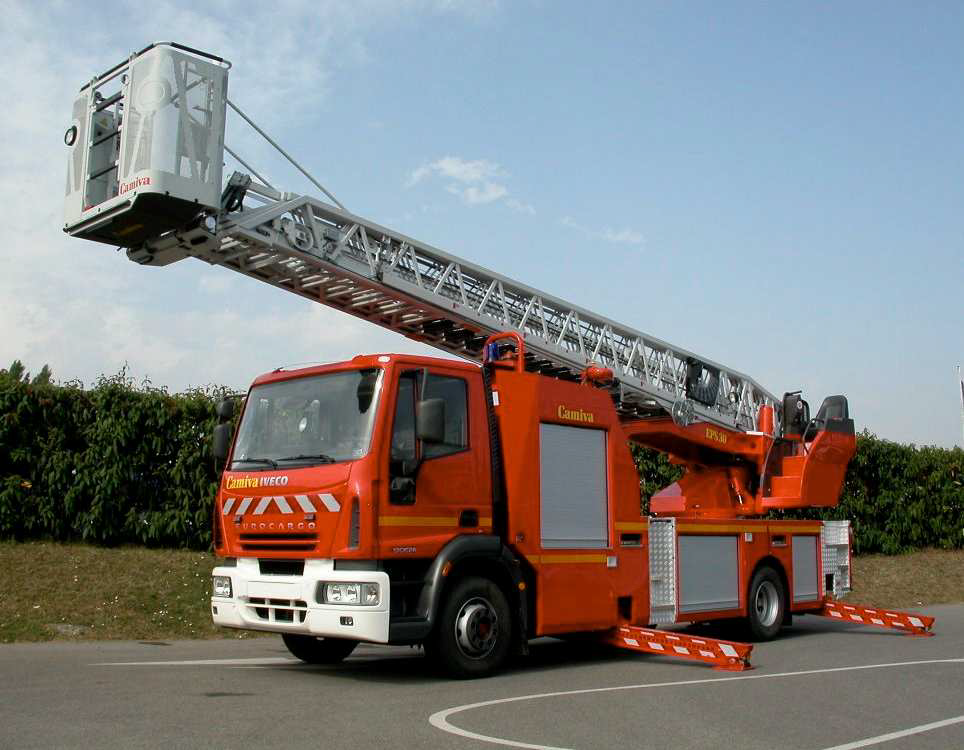
\includegraphics[width=.85\textwidth]{png/fig1}
\end{center}
\end{minipage} \hfill
\begin{minipage}[c]{.47\linewidth}
Une E.P.A.S. est une Échelle Pivotante Automatique à commande Séquentielle.
Ce système conçu et commercialisé par la société CAMIVA est monté sur le châssis d’un camion
de pompiers et permet de déplacer une plate-forme pouvant recevoir deux personnes et un brancard.

Ce système est constitué : 
\begin{itemize}
\item de deux tourelles;
\item de vérins permettant le déplacement des tourelles;
\item d'un berceau; 
\item d'un parc-échelle  et d'une plate forme.
\end{itemize}

\end{minipage}

%\vfill{}
%\begin{flushright}
%\textit{\footnotesize{Appelle au feu les pompiers...}}
%\end{flushright}

\begin{center}
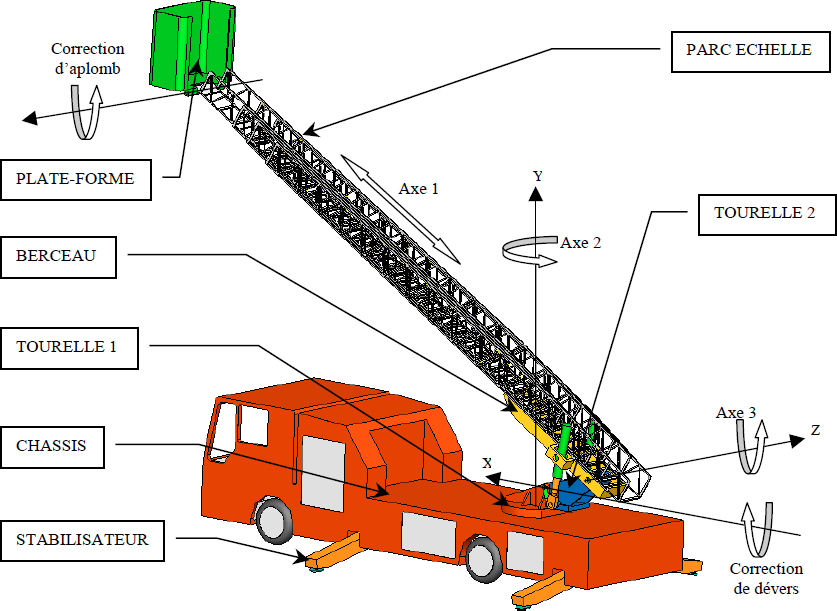
\includegraphics[width=.8\textwidth]{png/fig2}
\end{center}
Le déplacement de la plate-forme est réalisé suivant trois axes :
\begin{itemize}
\item le déploiement du parc échelle (axe 1) : Chaque plan de l’échelle peut se translater par
rapport aux autres ; seul le quatrième plan d’échelle est solidaire du berceau.
\item le pivotement autour de l’axe $\vect{z}$ (axe 2) : La tourelle 1 peut pivoter par rapport au
châssis autour d’un axe vertical.
\item la rotation autour de l’axe $\vect{z}$ (axe 3) : Le berceau peut tourner par rapport à la tourelle
2 autour d’un axe horizontal.
\end{itemize}
Pour garantir la sécurité, le système maintient toujours la plate forme en position horizontale :
\begin{itemize}
\item la correction d’aplomb oriente la plate-forme autour d’un axe horizontal parallèle à
l’axe $\vect{z}$;
\item la correction de devers oriente l’ensemble parc échelle et plate-forme autour de l’axe
$\vect{x}$ : la tourelle 2 s’oriente par rapport à la tourelle 1 suivant un axe perpendiculaire aux
axes 3 et 2.
\end{itemize}
Lors des déplacements suivant les axes 2 et 3, le système « VARIMAX » de commande des
actionneurs maintient la vitesse de la plate-forme la plus constante possible afin de limiter les
mouvements de balancier qui résulteraient d’une commande trop « brusque ».

On donne un extrait du diagramme des exigences et du cahier des charges fonctionnel.

%\vfill{}
%\begin{flushright}
%\textit{\footnotesize{Et tout Rio qui se réveille...}}
%\end{flushright}


\begin{center}
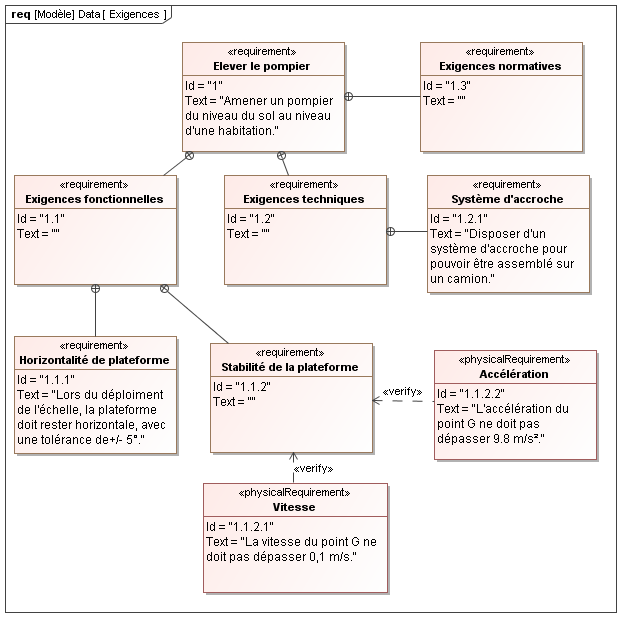
\includegraphics[width=.7\textwidth]{png/Exigences}
\end{center}


\begin{center}
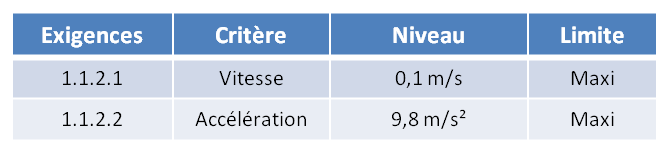
\includegraphics[width=.6\textwidth]{png/cdcf}
\end{center}
}

\section{Paramétrage du système}
\ifthenelse{\boolean{prof}}{}{
Le schéma cinématique du système ainsi que le paramétrage sont indiqués ci-après.

\begin{center}
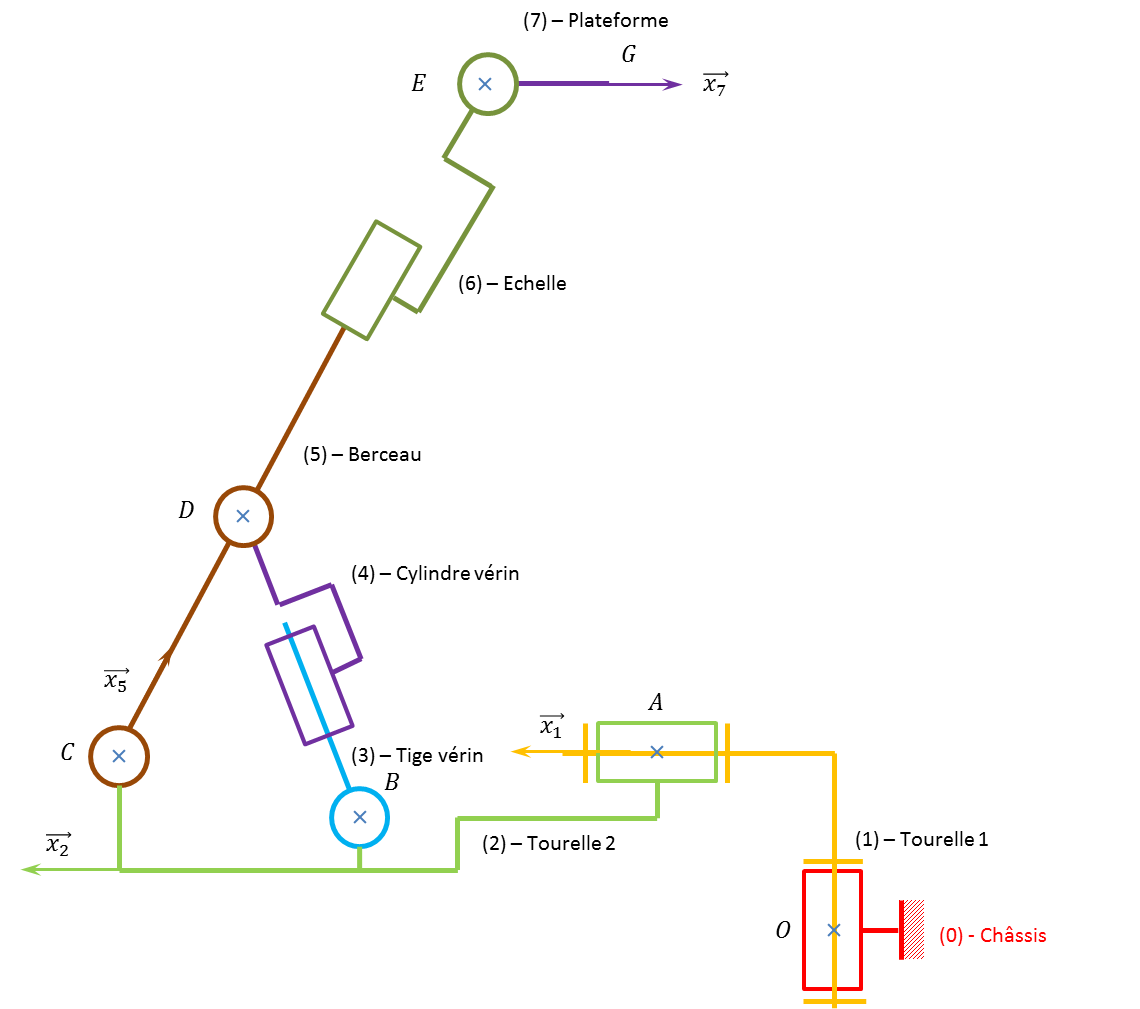
\includegraphics[width=.7\textwidth]{png/fig6}
\end{center}

\begin{center}
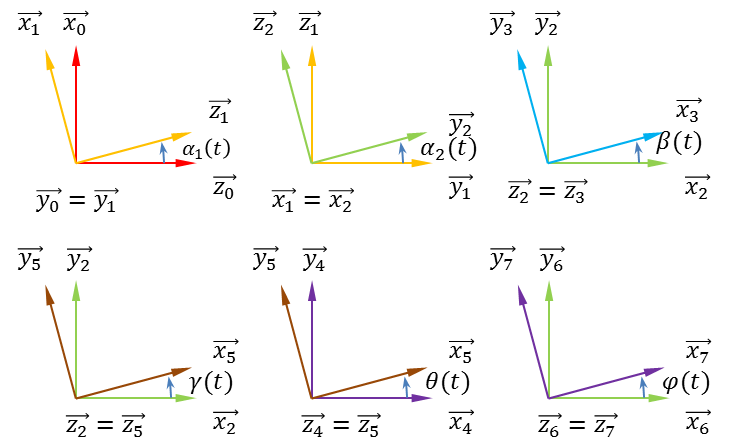
\includegraphics[width=.7\textwidth]{png/fig5}
\end{center}

Les pièces 5 et 6 étant en liaison glissière, on a donc $\vect{x_5}=\vect{x_6}$, $\vect{y_5}=\vect{y_6}$ et $\vect{z_5}=\vect{z_6}$.

Par ailleurs on donne :

\begin{minipage}[c]{.3\linewidth}
\begin{itemize}
\item $\vect{OA}=a\vect{y_1}+b\vect{x_1}$
\item $\vect{AB}=b\vect{x_2}-a\vect{y_2}$
\item $\vect{BC}=b\vect{x_2}+a\vect{y_2}$
\item $\vect{CD}=g\vect{x_5}$
\end{itemize}
\end{minipage}\hfill 
\begin{minipage}[c]{.45\linewidth}
\begin{itemize}
\item $\vect{BD}=\lambda(t)\vect{x_3}$
\item $\vect{DE}=\mu(t)\vect{x_6}$
\item $\vect{EG}=h\vect{x_7}$
\end{itemize}
\end{minipage}

%\vfill{}
%\begin{flushright}
%\textit{\footnotesize{Voit brûler l'usiner à café ...}}
%\end{flushright}


}
\section{Loi de commande dans le vérin}

L'élévation de la grue est donnée par l'allongement du vérin constitué des pièces 4 et 5. 

\subparagraph{}
\textit{Donner le graphe des liaisons constitués par les pièces 2, 3, 4, et 5. Comment appelle-t-on ce type de chaîne ?}
\ifthenelse{\boolean{prof}}{
\begin{corrige}
Le tracé du graphe des liaisons donne une chaîne fermée.
\end{corrige}
}{}

%\vfill{}

%\begin{flushright}
%\textit{\footnotesize{Il n'y a plus de temps à perdre ...}}
%\end{flushright}


\subparagraph{}
\textit{L'élévation de la grue est donnée par l'angle $\gamma(t)$ du berceau 5 par rapport à la tourelle 2. Réaliser une fermeture cinématique liant les solides 2, 3, 4 et 5 et donner une relation 
entre $\lambda$ et $\gamma$. %On pourra par exemple montrer que 
%$$
%\lambda(t)^2 = b^2 + g^2 +a^2 +2g\left( b\cos\gamma(t) a\sin\gamma(t)\right)
%$$}
}
\ifthenelse{\boolean{prof}}{
\begin{corrige}
Les solides 2, 3, 4 et 5 forment une chaîne fermée. La fermeture géométrique est la suivante : 
$$
\vect{BC}+\vect{CD}+\vect{DB} = \vect{0}
$$

$$
b\vect{x_2}+a\vect{y_2}+ g\vect{x_5}-\lambda(t)\vect{x_3} = \vect{0} 
$$
$$
\Longleftrightarrow
b\vect{x_2}+a\vect{y_2}+ g\cos\gamma\vect{x_2}+g\sin\gamma\vect{y_2}
-\lambda(t)\cos\beta\vect{x_2}-\lambda(t)\sin\beta\vect{y_2} = \vect{0} 
$$

On projette ensuite les expressions sur $\vect{x_2}$ et $\vect{y_2}$ :
$$
\left\{
\begin{array}{l}
b+ g\cos\gamma-\lambda(t)\cos\beta = 0  \\
a+ g\sin\gamma-\lambda(t)\sin\beta = 0 
\end{array}
\right.
$$
 
Il nous faut éliminer $\beta$ dans l'équation : 
$$
\left\{
\begin{array}{l}
\lambda(t)\cos\beta = b+ g\cos\gamma \\
\lambda(t)\sin\beta = a+ g\sin\gamma 
\end{array}
\right.
$$

En élevant les deux équations au carré et en les sommant on a donc : 
$$
\lambda(t)^2 = b^2 + g^2 \cos^2 \gamma + 2bg\cos\gamma + a^2 + g^2 \sin^2 \gamma + 2ag\sin\gamma 
$$

$$
\lambda(t)^2 = b^2 + g^2 + 2bg\cos\gamma + a^2 + 2ag\sin\gamma 
\Longleftrightarrow
\lambda(t)^2 = b^2 + g^2 + a^2 + 2g\left( b\cos\gamma + a\sin\gamma \right)
$$

\end{corrige}
}{}





\subparagraph{}
\textit{En faisant l'hypothèse que $b=g$ et $a=0$, exprimer $\gamma(t)$ en fonction de $\lambda(t)$ puis calculer $\dfrac{d\gamma(t)}{dt}$.}
\ifthenelse{\boolean{prof}}{
\begin{corrige}
En tenant compte des hypothèses précédentes : 
$$
\lambda(t)^2 = 2b^2  + 2b^2 \cos\gamma 
\Longleftrightarrow
\gamma = \arccos\left( \dfrac{\lambda(t)^2}{2b^2} - 1 \right)
$$

On a donc :
$$
\dot{\gamma} =
-\dfrac{\dfrac{\dot{\lambda}\lambda}{b^2}}{\sqrt{1-\left( \dfrac{\lambda(t)^2}{2b^2} - 1 \right)^2}}
=
-\dfrac{\dfrac{\dot{\lambda}\lambda}{b^2}}{\sqrt{-\dfrac{\lambda(t)^4}{4b^4}+\dfrac{\lambda(t)^2}{b^2} }}
$$
$$
\dot{\gamma} 
=-\dfrac{\dfrac{\dot{\lambda}}{b}}{\sqrt{1-\dfrac{\lambda(t)^2}{4b^2}}}
= -\dfrac{\dfrac{\dot{\lambda}}{b}}{\sqrt{\dfrac{4b^2-\lambda(t)^2}{4b^2} }}
= -\dfrac{\dot{\lambda}}{\dfrac{b}{2b}\sqrt{4b^2-\lambda(t)^2 }}
= -\dfrac{2\dot{\lambda}}{\sqrt{4b^2-\lambda(t)^2 }}
$$

\end{corrige}
}{}


%\subparagraph{}
%\textit{Donner les torseurs cinématiques suivants : 
%\begin{itemize}
%\item $\torseurcin{V}{3}{2}$ au point $B$;
%\item $\torseurcin{V}{4}{3}$ au point $B$ (on ne prendra pas en compte le pivotement de cette liaisons; en conséquence elle sera considérée comme une liaison glissière); 
%\item $\torseurcin{V}{5}{4}$ au point $D$ puis au point $B$;
%\item $\torseurcin{V}{2}{5}$ au point $C$ puis au point $B$;
%\end{itemize}
%}

%\subparagraph{}
%\textit{Expliquer \textbf{en moins de deux lignes} que 
%$\torseurcin{V}{2}{5}+\torseurcin{V}{5}{4}+\torseurcin{V}{4}{3}+\torseurcin{V}{2}{2}=\left\{ 0\right\}$ où $\left\{ 0\right\}$ désigne le torseur nul.}

%\subparagraph{}
%\textit{Appliquer le calcul.}

%\subparagraph{}
%\textit{}

\section{Élévation de la plateforme}

\textbf{On considère dans cette partie que $\alpha_{2}=0$.}

\textbf{Dans les calculs suivants, on ne tiendra pas compte des pièces 3 et 4.}

\subparagraph{}
\textit{Donner le graphe des liaisons du mécanisme en tenant compte des hypothèses ci-dessus. Comment appelle-t-on ce type de chaîne ?}
\ifthenelse{\boolean{prof}}{
\begin{corrige}
Le graphe des liaisons forme une chaîne ouverte.
\end{corrige}
}{}

\subparagraph{}
\textit{On souhaite que pendant le mouvement d'élévation, la plateforme reste horizontale. Donner la relation simple liant $\varphi(t)$ et $\gamma(t)$.}
\ifthenelse{\boolean{prof}}{
\begin{corrige}
La plate forme restera horizontale (si on suppose le tourelle 2 horizontale) si et seulement si : 
$$
\vect{x_7}\wedge \vect{x_2} = \vect{0} 
\Longleftrightarrow \sin\left( \varphi + \gamma \right) \vect{z_0}= \vect{0} 
\Longleftrightarrow  \varphi + \gamma = 0
$$

\end{corrige}
}{}

\subparagraph{}
%\textit{Donner le torseur cinématique $\torseurcin{V}{7}{6}$ au point $G$.}
\textit{Donner les vecteurs $\vecto{7}{6}$ et  $\vectv{G}{7}{6}$.}
\ifthenelse{\boolean{prof}}{
\begin{corrige}

$$
\torseurcin{V}{7}{6} = 
\torseurl{\vecto{7}{6}= \dot{\varphi}\vect{z_6}}{\vectv{G}{7}{6} = \underbrace{\vectv{E}{7}{6}}_{\vect{0}} + \vect{GE}\wedge\vecto{7}{6}}{G}
$$

$$\vectv{G}{7}{6} =-h\vect{x_7}\wedge\dot{\varphi}\vect{z_6} =h\dot{\varphi}\vect{y_7}
$$

$$
\torseurcin{V}{7}{6} = 
\torseurl{\vecto{7}{6}= \dot{\varphi}\vect{z_6}}{\vectv{G}{7}{6} = 
h\dot{\varphi}\vect{y_7}}{G}
$$
\end{corrige}
}{}

\subparagraph{}
%\textit{Donner le torseur de cinématique $\torseurcin{V}{6}{5}$ au point $G$.}
\textit{Donner les vecteurs $\vecto{6}{5}$ et  $\vectv{G}{6}{5}$.}
\ifthenelse{\boolean{prof}}{
\begin{corrige}

$$
\torseurcin{V}{6}{5} = 
\torseurl{\vecto{6}{5}= \vect{0}}{\vectv{G}{6}{5} = \dot{\mu}\vect{x_6}}{G}
$$


\end{corrige}
}{}


\subparagraph{}
\textit{On rappelle que $\mathcal{R}_5=\mathcal{R}_6$. Calculer les produits vectoriels suivants : $\vect{x_6}\wedge\vect{y_1}$, $\vect{y_6}\wedge\vect{y_1}$, $\vect{x_7}\wedge\vect{y_1}$.}
\ifthenelse{\boolean{prof}}{
\begin{corrige}

Calculons $\vect{x_6}\wedge\vect{y_1}=\vect{x_5}\wedge\vect{y_1}=\cos\gamma \vect{z_1}$.

Calculons $\vect{y_6}\wedge\vect{y_1}=\vect{y_5}\wedge\vect{y_1}=\left(\cos\gamma\vect{y_1} - \sin \gamma \vect{x_1}\right)\wedge\vect{y_1}=-\sin\gamma\vect{z_1}$.

Calculons $\vect{x_7}\wedge\vect{y_1}
=\left(\cos\varphi(t)\vect{x_6} + \sin\varphi(t)\vect{y_6} \right)\wedge\vect{y_1}
=\cos\varphi\cos\gamma\vect{z_1} -\sin\gamma \sin\varphi(t)\vect{z_1}
=\cos\varphi\cos\gamma\vect{z_1} -\sin\gamma \sin\varphi(t)\vect{z_1}
=\cos\left( \varphi + \gamma\right)\vect{z_1} $.

\end{corrige}
}{}

\subparagraph{}
%\textit{Donner le torseur de cinématique $\torseurcin{V}{2}{0}$ au point $G$.}
\textit{Donner les vecteurs $\vecto{2}{0}$ et  $\vectv{G}{2}{0}$.}
\ifthenelse{\boolean{prof}}{
\begin{corrige}

$$
\torseurcin{V}{2}{0} = 
\torseurl{\vecto{2}{0}= \dot{\alpha_1}\vect{y_1}}{%
\vectv{G}{2}{0} = \underbrace{\vectv{O}{2}{0}}_{\vect{0}} + \vect{GO}\wedge\vecto{2}{0}}{G}
$$

$$
\vect{GO}=\vect{GE}+\vect{ED}+\vect{DC}+\vect{CB}+\vect{BA}+\vect{AO}
=-h\vect{x_7}-\mu(t)\vect{x_6}-g\vect{x_5}-b\vect{x_2}-a\vect{y_2}-b\vect{x_2}+a\vect{y_2}-a\vect{y_1}-b\vect{x_1}
$$

$$
\vect{GO}
=-h\vect{x_7}-\mu(t)\vect{x_6}-g\vect{x_5}-3b\vect{x_2}-a\vect{y_2}
$$

$$
\vectv{G}{2}{0} =
\vect{GO}\wedge\dot{\alpha_1}\vect{y_1}=
-h\dot{\alpha_1}\cos\left(\varphi+\gamma\right)\vect{z_1}
-\mu(t)\dot{\alpha_1}\cos\gamma\vect{z_1}
-g\dot{\alpha_1}\cos\gamma\vect{z_1}
-3b\dot{\alpha_1}\vect{z_2}
$$

$$
\vectv{G}{2}{0} =
-\dot{\alpha_1}\left( 
h\cos\left(\varphi+\gamma\right)
+\left(\mu(t)+g\right)\cos\gamma
+3b
\right)\vect{z_1}
$$


$$
\torseurcin{V}{2}{0} = 
\torseurl{\vecto{2}{0}= \dot{\alpha_1}\vect{y_1}}{%
\vectv{G}{2}{0} = 
-\dot{\alpha_1}\left( 
h\cos\left(\varphi+\gamma\right)
+\left(\mu(t)+g\right)\cos\gamma
+3b
\right)\vect{z_1}
}{G}
$$
\end{corrige}
}{}


\subparagraph{}
\textit{On donne : $\vecto{5}{2}= \dot{\gamma}\vect{z_2}$ et 
$\vectv{G}{5}{2} = 
\left(g+\mu(t)\right)\dot{\gamma}\vect{y_5}+g\dot{\gamma}\vect{y_7}$. 
%\torseurcin{V}{5}{2} = 
%\torseurl{\vecto{5}{2}= \dot{\gamma}\vect{z_2}}{\vectv{G}{5}{2} = 
%\left(g+\mu(t)\right)\dot{\gamma}\vect{y_5}+g\dot{\gamma}\vect{y_7}}{G}
%$$
En déduire $\vecto{7}{0}$ et  $\vectv{G}{7}{0}$.}

\ifthenelse{\boolean{prof}}{
\begin{corrige}
$$\vecto{7}{0} = \vecto{7}{5}+\vecto{5}{2}+\vecto{2}{0}$$ 
$$\vectv{G}{7}{0} = \vectv{G}{7}{5}+\vectv{G}{5}{2}+\vectv{G}{2}{0}$$ 
\end{corrige}
}{}

%\vfill{}
%\begin{flushright}
%\textit{\footnotesize{Sinon tout le quartier va brûler...}}
%\end{flushright}

\subparagraph{}
\textit{Dans le cas où $\alpha_1$ et $\mu$ sont des constantes, on a 
$\vectv{G}{7}{0} =
h\dot{\varphi}\vect{y_7}
+\left(g+\mu(t)\right)\dot{\gamma}\vect{y_5}+g\dot{\gamma}\vect{y_7}$. 
Calculer alors $\vectg{G}{7}{0}$.}
\ifthenelse{\boolean{prof}}{
\begin{corrige}

$$
\vectg{G}{7}{0} =
h\ddot{\varphi}\vect{y_7}+h\dot{\varphi}\left[\dfrac{d\vect{y_7}}{dt}\right]_{\mathcal{R}_0}
+\left(g+\mu(t)\right)\ddot{\gamma}\vect{y_5}
+\left(g+\mu(t)\right)\dot{\gamma}\left[\dfrac{d\vect{y_5}}{dt}\right]_{\mathcal{R}_0}
+g\ddot{\gamma}\vect{y_7}
+g\dot{\gamma}\left[\dfrac{d\vect{y_7}}{dt}\right]_{\mathcal{R}_0}
$$


Commençons par calculer les dérivées de vecteurs :
$$
\left[\dfrac{d\vect{y_7}}{dt}\right]_{\mathcal{R}_0}
=
\left[\dfrac{d\vect{y_7}}{dt}\right]_{\mathcal{R}_7}
+\vecto{7}{0}\wedge\vect{y_7}
=\left(\dot{\varphi}\vect{z_6} + \dot{\gamma}\vect{z_5}\right) \wedge\vect{y_7}
=-\left(\dot{\varphi}+\dot{\gamma}\right)\vect{x_7} 
$$

$$
\left[\dfrac{d\vect{y_5}}{dt}\right]_{\mathcal{R}_0}
=
\left[\dfrac{d\vect{y_5}}{dt}\right]_{\mathcal{R}_5}
+\vecto{5}{0}\wedge\vect{y_5}
= \dot{\gamma}\vect{z_5} \wedge\vect{y_5}
= -\dot{\gamma}\vect{x_5} 
$$

On a donc : 
$$
\vectg{G}{7}{0} =
h\ddot{\varphi}\vect{y_7}
-h\dot{\varphi}\left(\dot{\varphi}+\dot{\gamma}\right)\vect{x_7} 
+\left(g+\mu(t)\right)\ddot{\gamma}\vect{y_5}
-\left(g+\mu(t)\right)\dot{\gamma}^2\vect{x_5} 
+g\ddot{\gamma}\vect{y_7}
-g\dot{\gamma}\left(\dot{\varphi}+\dot{\gamma}\right)\vect{x_7} 
$$

$$
\vectg{G}{7}{0} =
\left(h\ddot{\varphi}+g\ddot{\gamma}\right)\vect{y_7}
-\left(h\dot{\varphi}+g\dot{\gamma} \right)\left( \dot{\varphi}+\dot{\gamma}\right)\vect{x_7} 
+\left(g+\mu(t)\right)\ddot{\gamma}\vect{y_5}
-\left(g+\mu(t)\right)\dot{\gamma}^2\vect{x_5} 
$$

\end{corrige}
}{}

\section{Validation du cahier des charges}
\subparagraph{}
\textit{A l'aide de l'étude réalisée ci-dessus, donner une méthode permettant de vérifier que les exigences 1.1.2.1 et 1.1.2.2 sont satisfaites.}% On considèrera pour cela que $\mu=20m$, $\dot{\gamma}$ (et donc $\dot{\varphi}$), $\alpha_1$ et $\alpha_2$ sont des constantes; $g=b=h=0,5m$; $a=0 m$; $\dot{\lambda}=10mm/s$ }

\ifthenelse{\boolean{prof}}{
\begin{corrige}
Un certain nombre d'hypothèses serait nécessaire pour répondre à cette question :
\begin{itemize}
\item on peut d'abord faire l'hypothèse que le déploiement du vérin suit une loi en trapèze de vitesse. On peut donc avoir $\lambda(t)$ et $\dot{\lambda}(t)$;
\item la loi entrée-sortie permet alors d'avoir $\gamma(t)$,  $\dot{gamma}(t)$ et $\ddot{gamma}(t)$;
\item une relation entre $\gamma$ et $\varphi(t)$ a été donnée ultérieurement;
\item on fait l'hypothèse que $\alpha_1$ et $\alpha_2$ sont des constantes (ce qui peut se justifier car ces angles correspondent au réglage de l'assiette du camion).
\end{itemize}
Il faudrait ensuite calculer les normes de la vitesse et de l'accélération (après avoir projeté les vecteurs dans une base donnée).
Connaissant les différentes constantes, on pourrait alors tracer l'allure les courbes de vitesse et d'accélération et vérifier que les CDCF est vérifié.
\end{corrige}
}{}


\end{document}



\subparagraph{}
\textit{}
\ifthenelse{\boolean{prof}}{
\begin{corrige}
\end{corrige}
}{}





\ifthenelse{\boolean{prof}}{
\begin{corrige}
On a $\vectv{G}{7}{0} =\left( h\dot{\varphi}+ g\dot{\gamma}\right)\vect{y_7}
+\left(g+\mu(t)\right)\dot{\gamma}\vect{y_5}$. Par ailleurs, $\vect{y_7}=\cos \varphi \vect{y_6}-\sin \varphi \vect{x_6}=\cos \varphi \vect{y_5}-\sin \varphi \vect{x_5}$. 

On a donc :
\begin{eqnarray*}
\vectv{G}{7}{0} &=&\left( h\dot{\varphi}+ g\dot{\gamma}\right)\left( \cos \varphi \vect{y_5}-\sin \varphi \vect{x_5}\right)
+\left(g+\mu(t)\right)\dot{\gamma}\vect{y_5} \\
&=& 
-\sin \varphi \left( h\dot{\varphi}+ g\dot{\gamma} \right)\vect{x_5}+ \left(\left(h\dot{\varphi} + g\dot{\gamma}\right)\cos \varphi +\left(g+\mu(t)\right)\dot{\gamma} \right)\vect{y_5}
\end{eqnarray*}


On a donc :

\begin{eqnarray*}
\vectv{G}{7}{0}^2 &=& \left( h\dot{\varphi}+ g\dot{\gamma} \right)^2\sin ^2\varphi+
\left(\left(h\dot{\varphi} + g\dot{\gamma}\right)\cos \varphi +\left(g+\mu(t)\right)\dot{\gamma} \right)^2 \\
&=& \left( h\dot{\varphi}+ g\dot{\gamma} \right)^2\sin ^2\varphi+
\left(h\dot{\varphi} + g\dot{\gamma}\right)^2\cos^2 \varphi +\left(g+\mu(t)\right)^2\dot{\gamma} ^2  + 2 \left(
\left(h\dot{\varphi} + g\dot{\gamma}\right)\cos\varphi \cdot\left(g+\mu(t)\right)\dot{\gamma}  \right)\\
&=& \left( h\dot{\varphi}+ g\dot{\gamma} \right)^2 +\left(g+\mu(t)\right)^2\dot{\gamma} ^2  + 2 \left(
\left(h\dot{\varphi} + g\dot{\gamma}\right)\cos\varphi \cdot\left(g+\mu(t)\right)\dot{\gamma}  \right)\\
\end{eqnarray*}

Par ailleurs on a vu que 
$\dot{\gamma} = -\dfrac{2\dot{\lambda}}{\sqrt{4b^2-\lambda(t)^2 }}$.
\end{corrige}
}{}




\end{document}



\subparagraph{}
\textit{}
\ifthenelse{\boolean{prof}}{
\begin{corrige}
\end{corrige}
}{}

